\section{Architektura}

Stroje,
které sestavují či spouštejí aplikace,
nezajímá vzhled či uspořádání zdrojového kódu.
Naopak vývojáři,
jakožto lidé,
potřebují udržovat kód snadno čitelný a~srozumitelně rozdělený do jednotlivých
metod, tříd, struktur či vrstev aplikace.
Potřebují také vysokoúrovňové jazyky či pokročilé knihovny a~frameworky,
které ulehčí psaní kódu a~nenutí vývojáře psát vše znovu.
I~přes to ale nejsou aplikace psány dle nejlepších doporučení
a~vývojáři velmi často píší či naráží na tak zvaný \uv{spaghetti code}~\cite{architecture}.
To je mnohdy zapříčiněno nárokem na rychlou implementaci nových funkcí či úprav,
kde vývojáři na úkor času zanedbají čitelnost a~strukturu kódu
a~čím dál tím více postupem času prohlubují dluh kvality daného kódu.
\emph{\uv{Software has two types of value:
        the~value of its behavior and the~value of its structure.
        The~second of these is the~greater of the~two
        because it is this value that makes
        software soft.}}~\cite[str.~140]{martin_clean_architecture}
Ze zmíněného zdroje také plyne,
že se dlouhodobě vyplatí vývoj směřovat k~dobré struktuře a~architektuře,
než k~samotné implementaci,
jelikož implementace se snadno opraví,
kdežto opravit architekturu bez velkého zásahu
je značně obtížné~\cite[str.~135--146]{martin_clean_architecture}.

Cílem každé aplikace je mít udržitelný a~snadno rozšiřitelný kód.
Je proto třeba stanovit řadu pravidel,
které pomohou s~vývojovými otázkami při návrhu metod, tříd, rozhraní či
celých modulů.
Architektura a~její správný a~\mbox{promyšlený} návrh umožňuje vyvarovat
se chyb a~dluhu na kvalitě a~modularitě,
který znemožní snadný proces udržitelnosti aplikace.
\emph{\uv{Good \mbox{architecture} makes the~system easy to~understand,
easy to~develop, easy to~maintain, and~easy to~deploy.
The~ultimate goal is to~minimize the~lifetime cost of~the~system
and~to~maximize programmer productivity.}}~\cite[str.~137]{martin_clean_architecture}
Dobře navržená a~udržovaná architektura tak umožní z~dlouhodobého hlediska
produkovat kvalitnější kód~\cite[str.~135--146]{martin_clean_architecture}.
Kvalitnější architektura tedy logicky minimalizuje nutnost oprav
a~přizpůsobení struktury aplikace při vývoji každé nové funkcionality.

Dle zdroje~\cite{architecture} lze rozdělit architektury do dvou skupin:
architektury zaměřené na databázi a~architektury zaměřené na doménu.
V~následujících sekcích budou popsány rozdíly mezi oběma skupinami
a~vybranými konkrétními případy architektur.

\subsection{Architektury zaměřené na databázi}

Architektury zaměřené na databázi,
také nazývané \emph{database-centric architectures},
byly dle~\cite{architecture} prvním typem softwarových architektur.
Tyto architektury staví databáze do středu dění,
jak jde vidět z~obrázku~\ref{fig:architecture_database}.

\begin{figure}
    \centering
    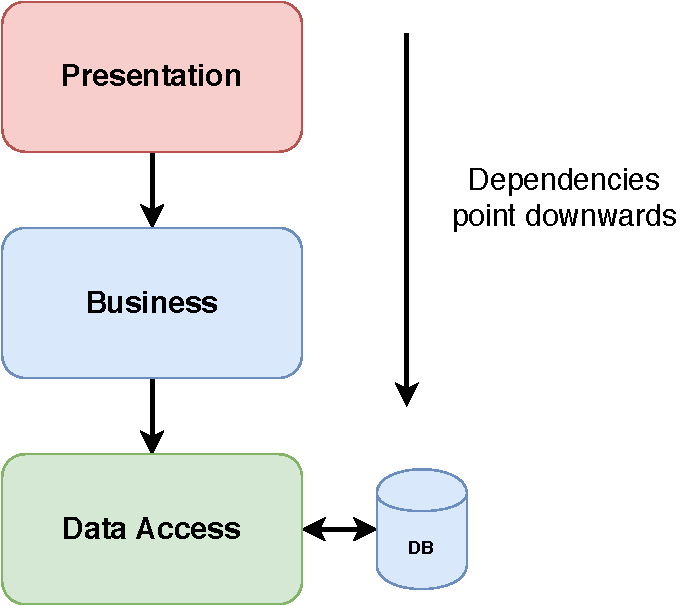
\includegraphics[width=0.5\linewidth]{assets/technology-research/architecture/database-centric.pdf}
    \caption{Schéma architektury zaměřené na databázi~\cite{architecture}}
    \label{fig:architecture_database}
\end{figure}

Příkladem tohoto typu architektury je tradiční 3-vrstvá architektura.
Ta je robustní a~škálovatelná.
Skládá se ze tří vrstev.
První vrstva,
prezentační vrstva,
obsahuje tvorbu UI,
bez samotného kódu s~logikou.
Druhá vrstva,
aplikační vrstva,
obsahuje samotný kód s~logikou aplikace.
Tato vrstva by měla být nezávislá na prezentační vrstvě,
avšak má explicitní závislost na datové vrstvě.
Poslední vrstva,
datová vrstva,
je nejnižší vrstvou,
která se stará o~manipulaci a~tok dat z~databáze do
nižších vrstev.
V~této architektuře je největší role přikládána databázi
a~často je tak datová a~aplikační vrstva úzce propojena.
V~nejhorších případech na datové vrstvě závisí
i~vrstva prezentační~\cite{architecture}.
Ukázka přístupu pomocí této architektury je znázorněna ve výpisu
kódu~\ref{code:architecture-database}.

\begin{listing}
    \caption{Ukázka přístupu zaměřeného na databázi v~jazyce Java~\cite{architecture}}
    \label{code:architecture-database}
    \begin{minted}{java}
package ua.com.crosp.testapp.domain;
import ua.com.crosp.testapp.datalayer.PostsRepository;

public class GetRecentPostsUseCase
implements GetRecentPostsUseCaseContract {
    private PostsRepository mPostsRepository;

    public Single<Post.List> execute(Params params) {
        // Execute
    }
}
    \end{minted}
\end{listing}



\subsection{Architektury zaměřené na doménu}

\begin{figure}
    \centering
    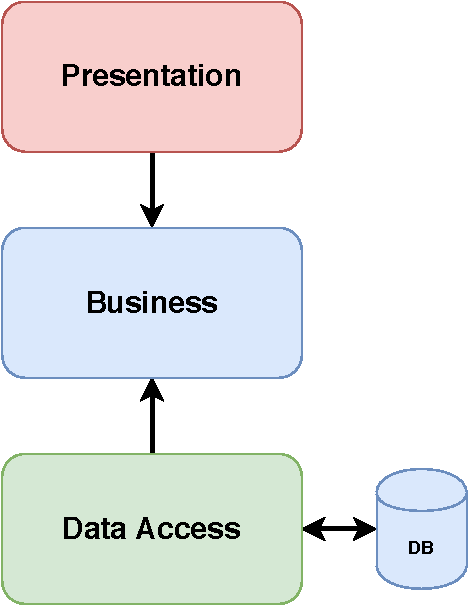
\includegraphics[width=0.35\linewidth]{assets/technology-research/architecture/domain-centric.pdf}
    \caption{Schéma architektury zaměřené na doménu~\cite{architecture}}
    \label{fig:architecture_domain}
\end{figure}

Architektury zaměřené na doménu,
také nazývané \emph{domain-centric architectures},
jsou produktem vývoje z~předchozího typu architektur.
Jak jde vidět z~obrázku~\ref{fig:architecture_domain},
střed dění je přesunut na aplikační vrstvu,
protože právě tato vrstva je v~aplikaci nejdůležitější,
jelikož v~ní probíhá implementace nových funkcionalit,
změn či oprav~\cite{architecture}.
\emph{\uv{The~way you keep software soft is
to~leave as~many options open as~possible,
for as~long as~possible.
What are the~options that we need to~leave open?
They are the~details
that don’t matter.}}~\cite[str.~140]{martin_clean_architecture}

Výhodou architektur zaměřených na doménu také je,
že díky návrhu samotnému abstrahují implementační detaily do podoby kontraktů.
Těmto kontraktům může nadále vyhovět několik konkrétních implementací,
což umožní snadnou výměnu služeb
či jiných závislostí~\cite[str.~135--146]{martin_clean_architecture}.
Lze tedy jednoduše nahradit například konkrétní databázi
--- z~databáze MySQL na databázi Cloud Firestore ---,
bez toho,
aniž by se muselo zasahovat do samotné aplikační vrstvy aplikace.
Ukázka přístupu pomocí tohoto typu architektury je znázorněna
ve výpisu kódu~\ref{code:architecture-domain}.

\begin{listing}
    \caption{Ukázka přístupu zaměřeného na doménu v~jazyce Java~\cite{architecture}}
    \label{code:architecture-domain}
    \begin{minted}{java}
package ua.com.crosp.testapp.domain;
import ua.com.crosp.testapp.domain.PostsRepositoryContract;

public class GetRecentPostsUseCase
implements GetRecentPostsUseCaseContract {
    private PostsRepositoryContract mPostsRepository;

    @Inject
    public GetRecentPostsUseCase(PostsRepositoryContract r) {
        mPostsRepository = r;
    }
    public Single<Post.List> execute(Params params) {
        // Execute
    }
}
    \end{minted}
\end{listing}

\subsection{Clean Architecture}

Clean Architecture je architektura popisovaná ve stejnojmenné knize
od\linebreak \mbox{Roberta~C. Martina}.
\emph{\uv{Good software systems begin with clean code.
On~the~one hand, if the~bricks aren’t well made,
the~architecture of~the~building doesn’t matter much.
On~the~other hand, you can make a~substantial mess with well-made bricks.
This is where the~SOLID principles
come in.}}~\cite[str.~57]{martin_clean_architecture}
\linebreak
Architektura hojně využívá principů SOLID,
které byly představeny stejným autorem jako kniha.
Principy SOLID jsou následující:

\begin{description}
    \item[Single-responsibility principle] \emph{\uv{An active corollary to 
Conway’s law:\linebreak
The~best structure for a~software system is heavily influenced
by the~social structure of the~organization that uses it so that
each software module has one, and only one, reason to change.}}~\cite[str.~57--59]{martin_clean_architecture}
    \pagebreak
    \item[Open--closed principle] \emph{\uv{Bertrand Meyer made this principle
famous\linebreak in~the~1980s.
The gist is that for software systems to be easy to change,
they must be designed to allow the behavior of those systems to be changed
by~adding new code,
rather than changing existing code.}}~\cite[str.~57--59]{martin_clean_architecture}
    \item[Liskov substitution principle] \emph{\uv{Barbara Liskov’s famous 
definition of subtypes, from~1988.
In short, this principle says that to build software systems from
interchangeable parts,
those parts must adhere to a~contract that allows those parts to be
substituted one for another.}}~\cite[str.~57--59]{martin_clean_architecture}
    \item[Interface segregation principle] \emph{\uv{This principle advises
software designers to avoid depending on things that they don’t use.}}~\cite[str.~57--59]{martin_clean_architecture}
    \item[Dependency inversion principle] \emph{\uv{The code that implements
high-level policy should not depend on the code that implements low-level
details.
Rather, details should depend on policies.}}~\cite[str.~57--59]{martin_clean_architecture}
\end{description}

\begin{figure}[h!]
    \centering
    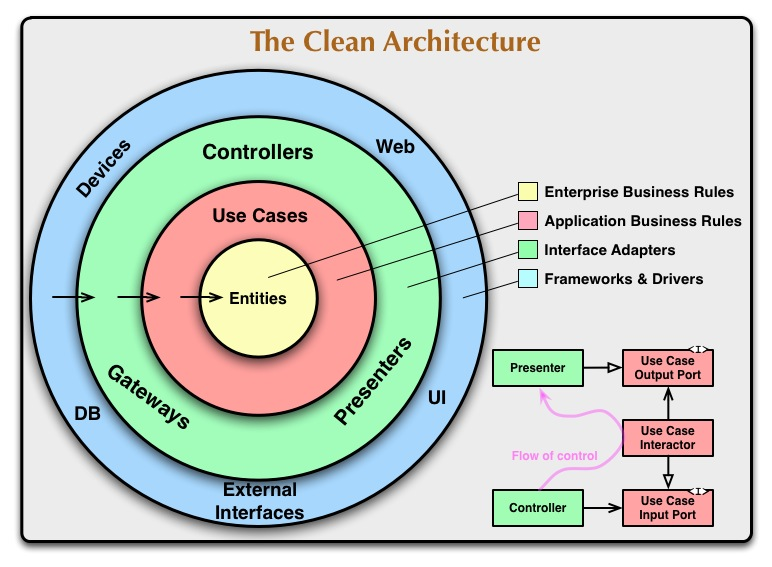
\includegraphics[width=\linewidth]{assets/technology-research/architecture/clean-architecture.jpg}
    \caption{Schéma architektury
        Clean Architecture~\cite{the_clean_architecture}}
    \label{fig:the_clean_architecture}
\end{figure}

\pagebreak
Princip inverze závislostí je jedním z~nejdůležitějších principů SOLID,
který Clean Architecture využívá.
Tento princip říká,
že by kód neměl záviset na detailech přímo,
ale raději na obecném kontraktu
(například pomocí dědičnosti nebo rozhraní),
který daný detail implementuje.
Další principy popisují,
že každá třída by měla mít zodpovědnost právě za jednu
věc,
rozšíření by mělo být možné pouze za pomoci přidání nového kódu,
pokud kód využívá třídu,
musí fungovat i~pokud místo ní použijeme její podtřídu
a~třídy by neměly záviset na více věcech,
než je potřeba~\cite[str.~61--91]{martin_clean_architecture}.
Obdobné principy jsou aplikovány i~na úrovni komponent aplikace
a~dohromady s~principy SOLID způsobí,
že takový systém je testovatelný,
nezávislý na konkrétním UI (web, mobilní zařízení, desktop),
použitém frameworku, použité databázi či dalších
službách~\cite{the_clean_architecture}.

Cílem architektury Clean Architecture je hlavně vhodné oddělení zodpovědnosti.
Jak jde vidět z~obrázku~\ref{fig:the_clean_architecture},
závislost jednotlivých vrstev aplikace může mířit pouze dovnitř.
Zároveň jsou věci uvnitř více abstraktní,
zatímco věci na kraji více konkrétní.
Středem všeho jsou entity,
které mohou obsahovat samotná data,
ale i~jejich funkce.
S~entitami pracují \emph{use cases},
které implementují za pomocí entit všechny případy užití.
Poslední vrstva většinou neobsahuje implentaci
a~pouze volá vnitřní vrstvu.
Do této vrstvy může patřit například mobilní framework (framework Flutter),
který volá kontroler (state management BLoC),
který zařídí pouze samotné spuštění správného use case.
Tato pravidla nejsou striktní a~už pouhým rozdělením do vhodných vrstev
či~pravidlem pro směr závislostí lze vytvořit velmi udržitelný
software.~\cite{the_clean_architecture}

\begin{figure}[t!]
    \centering
    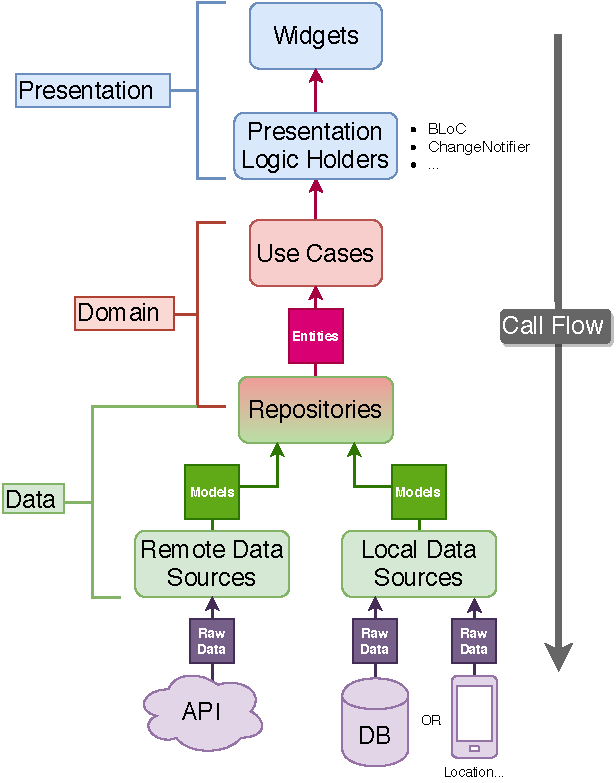
\includegraphics[width=0.85\linewidth]{assets/technology-research/architecture/reso-coder-clean-architecture.pdf}
    \caption{Schéma Reso Coder's Flutter Clean Architecture Proposal~\cite{reso_coder_clean_architecture}}
    \label{fig:reso_coder_clean_architecture}
\end{figure}

Otázka architektury je také dělení kódu do nezávislých sekcí či balíčků.
Přístupy se mohou lišit,
nejběžnějším je však rozdělení dle vrstev,
tedy nejčastěji dle prezentační, aplikační a~datové vrstvy.
Takovýto přístup je pro začátek dostačující a~často je doporučován tutoriály.
Dalším přístupem je rozdělení dle stejných vlastostí (\emph{features}).
To znamená,
že se kód nedělí horizontálně,
ale vertikálně.
Kód je sice možná lehčí nalézt,
než u~přístupu rozdělení dle vrstev,
avšak pro změnu neřeší oddělení dat, domény a~UI.
Dalším z~přístupů je rozdělení kódu jak dle vlastností,
tak následně dle vrstev,
což přináší výhody z~obou předešlých
způsobů.~\cite[str.~303--321]{martin_clean_architecture}

Tato architektura je samozřejmě značně abstraktní,
proto je nutné konkrétní věci organizovat dle potřeb aplikace,
například dle návrhu \emph{Reso Coder's Flutter Clean Architecture Proposal},
který je vidět na obrázku~\ref{fig:reso_coder_clean_architecture}.
Tento návrh rozděluje kód do vrstev tak,
že framework Flutter a~správa stavů je ve vrstvě prezenční,
use cases, entity a~kontrakty repozitířů jsou ve vrstvě aplikační
a~modely (které dědí z~entit) a~implementace repozitářů jsou ve vrstvě datové.
Třídy modelů oproti entitám obsahují transformační metody jako
převod z~a~do formátu JSON,
jelikož tyto metody jsou pro aplikační vrstvu nepodstatným
detailem.~\cite{reso_coder_clean_architecture}

\subsection{Zhodnocení}

Architektury zaměřené na databázi až příliš lpí na detailech,
na kterých ve výsledku nezáleží.
Architektury zaměřené na doménu tento problém naopak řeší,
využitím kontraktů namísto specifických detailů.
Architektura Clean Architecture je vhodným příkladem takovéto architektury.
Díky principům SOLID a~dalších vhodných pravidlech a~jejich využíváním
je možné lehce tvořit udržitelný a~rozšiřitelný kód,
ve kterém se lze snadno pohybovat a~vše má své dané místo.
V~praktické části bude proto využíváno právě architektury Clean Architecture.
